\clearpage

\section{Single Photon Receiver}

This block of code simulates the reception of two time continuous signals which are the outputs of single photon detectors and decode them in measurements results. A simplified schematic representation of this block is shown in figure \ref{SPR_receiver_block_diagram_simple}.

\begin{figure}[h]
	\centering
	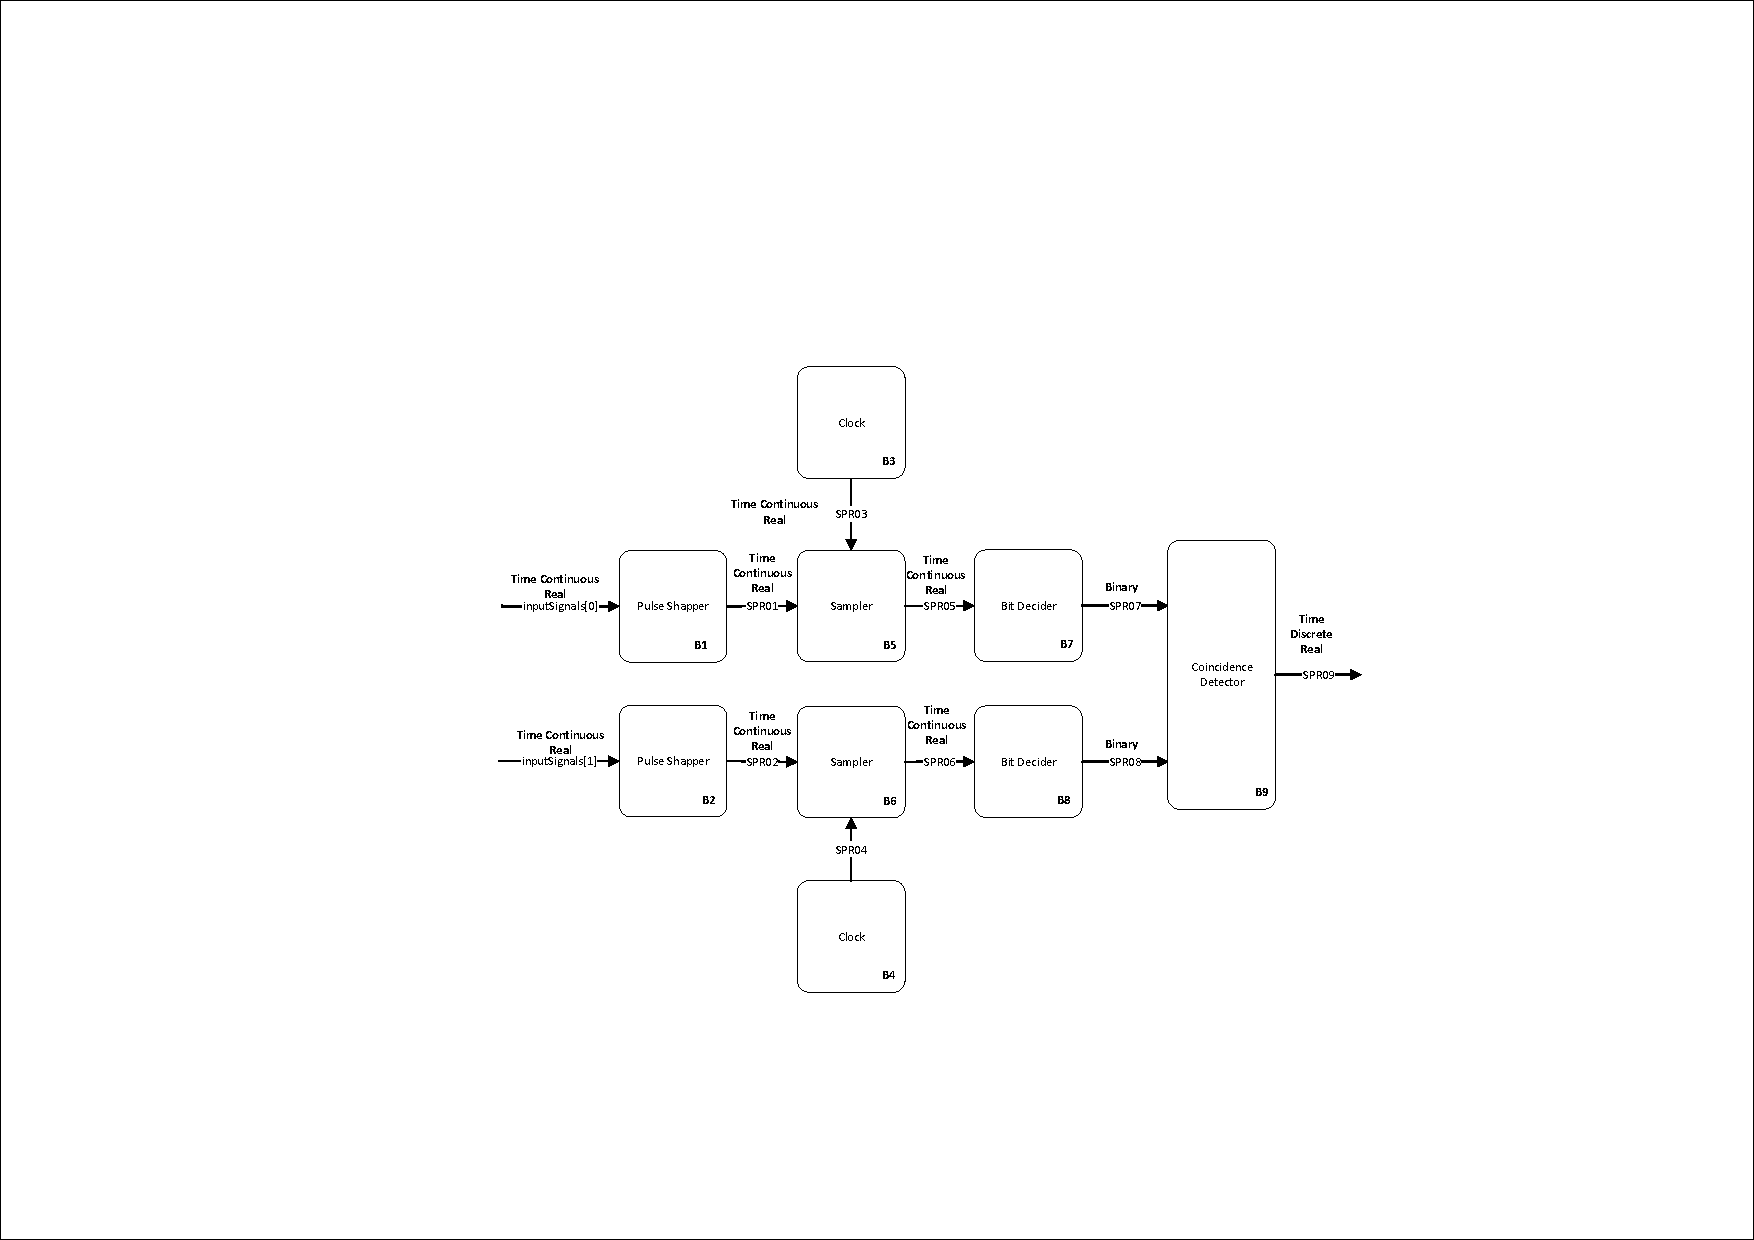
\includegraphics[clip, trim=8cm 4cm 6cm 5cm, width=1.00\textwidth]{../lib/single_photon_receiver/figures/single_photon_receiver.pdf}
	\caption{Basic configuration of the SPR receiver}\label{SPR_receiver_block_diagram_simple}
\end{figure}

\subsection*{Functional description}

This block accepts two time continuous input signals and outputs one time discrete signal that corresponds to the single photon detection measurements demodulation of the input signal. It is a complex block (as it can be seen from figure \ref{SPR_receiver_block_diagram_simple} of code made up of several simpler blocks whose description can be found in the \textit{lib} repository.

In can also be seen from figure \ref{SPR_receiver_block_diagram_simple} that there are two extra internal input signals generated by the \textit{Clock} in order to keep all blocks synchronized. This block is used to provide the sampling frequency to the \textit{Sampler} blocks.


\subsection*{Input parameters}

This block has some input parameters that can be manipulated by the user in order to change the basic configuration of the receiver. Each parameter has associated a function that allows for its change. In the following table (table~\ref{table}) the input parameters and corresponding functions are summarized.

\begin{table}[h]
	\begin{center}
		\begin{tabular}{| m{3,5cm} | m{5,8cm} |  m{2,5cm} | m{4cm} | }
			\hline
			\textbf{Input parameters} & \textbf{Function} & Type & \textbf{Accepted values} \\ \hline
			samplesToSkip            & Samples to skip in sampler block & int values\\
            filterType                  & Type of the filter applied in pulse shapper & PulseShaperFilter \\
            
			\hline
		\end{tabular}
		\caption{List of input parameters of the block SP receiver} \label{table}
	\end{center}
\end{table}

\pagebreak

\subsection*{Methods}

SinglePhotonReceiver(vector <Signal*> \&inputSignals, vector <Signal*> \&outputSignals)(\textbf\{constructor\})
\bigbreak
void setPulseShaperFilter(PulseShaperFilter fType)
\bigbreak
void setPulseShaperWidth(double pulseW)
\bigbreak
void setClockBitPeriod(double period)
\bigbreak
void setClockPhase(double phase) 
\bigbreak
void setClockSamplingPeriod(double sPeriod)
\bigbreak
void setThreshold(double threshold) 

\pagebreak

\subsection*{Input Signals}

\subparagraph*{Number:} 2

\subparagraph*{Type:} Time Continuous Amplitude Continuous Real

\subsection*{Output Signals}

\subparagraph*{Number:} 1

\subparagraph*{Type:} Time Discrete Amplitude Discrete Real

\subsection*{Example}

\subsection*{Sugestions for future improvement}
